\documentclass[11pt]{report}
\usepackage[paper=a4paper,margin=2.5cm]{geometry}
\usepackage{multicol}
\usepackage{fontspec}

% Point fontspec at your local fonts folder:
\setmainfont{EBGaramon}[
  Path      = font/,       % relative to main.tex
  Extension = .ttf,
  UprightFont    = *d12-Regular,   % MyFont-Regular.ttf
  BoldFont       = *d08-Regular,       % MyFont-Bold.ttf
  ItalicFont     = *d12-Italic,
  BoldItalicFont = *d08-Italic
]

\usepackage{microtype}
\usepackage{graphicx}
\usepackage[colorlinks,linkcolor=blue,urlcolor=cyan]{hyperref}
\usepackage{titlesec}
\titleformat{\chapter}[hang]{\normalfont\huge\bfseries}{}{0pt}{}
%=== Metadata ===
\newcommand{\thesistitle}{Your Thesis Title Here}
\newcommand{\authorname}{Rafael Tanzer}
\newcommand{\supervisor}{Michele Chiaria, Simone , Francesco Pontigia and Ezzio Bartocci}
\newcommand{\institution}{TU Vienna}
\newcommand{\department}{Cyber-Physical-Systems, ..., ...}
\newcommand{\logoimage}{graphics/logo.png} % Path to your logo image
\newcommand{\submissionmonth}{May}
\newcommand{\submissionyear}{2025}
%================

\usepackage[backend=biber, style=alphabetic]{biblatex}
\addbibresource{bibliography/theory.bib}

\begin{document}

\begin{titlepage}
  \centering
  \vspace*{1cm}

  % University logo
  
\includegraphics[width=0.25\textwidth]{graphics/tuWienLogo.png}
  \\[1cm]

  % Thesis title
  {\Huge \thesistitle\\[1.5cm]}

  % Project logo under title, smaller size
  \includegraphics[width=0.15\textwidth]{\logoimage}\\[1cm]

  % Author\maketitle
  {\Large \authorname\\[0.5cm]}

  % Department and institution
  {\large \department\\
  \institution\\[1.5cm]}

  % Supervisor
  {\large Supervisor: \supervisor\\[2cm]}

  % Submission date
  {\large \submissionmonth~\submissionyear\\}

  \vfill

  % Bottom of the page
  \vspace*{0.5cm}
  {\small This thesis is submitted in partial fulfillment of the requirements for the degree of \textit{Bachelor of Science}.}

\end{titlepage}


\begin{abstract}
  % Your abstract text here.
\end{abstract}

\tableofcontents

%=== Part I – Foundations ===%
\part{Foundations}

\chapter{Introduction}
\section{Motivation and Problem Statement}

CPS team - waht do they need it for
code growing user base - interconnecticty os , other qualities speaking for the usage of vs code
-
already in possesion of Haskell Checker but

\section{Objectives and Scope}
The main goal of the thesis was to create a \textit{Language Extension} ?NAME? for \textit{MiniProb}. Language extensions are a big part of
VS Code’s extension ecosystem and enable the editor to utilize custom language tooling. Such extensions support the user during the implementation process
while writing code, by providing language assistance like syntax validation or code completion. While this implementation targets VS Code, the underlying
logic and functionality are not limited to it — through the use of the \textit{Language Server Protocol (LSP)}, the developed tooling can be reused across
various editors and IDEs that support the protocol. The core functionality of these extensions stems from \textit{parsers} which, against a formal language
definition, convert written text into abstracted parts, validating the code in the process. These parts can then be used to extend the capabilities of the
tooling to encompass referential validation, type checking, code completion, diagnostics, and other language services that enhance the development experience.

In order for parsers to function accordingly, they require formal language definitions or models. These definitions range from various types of grammars to
abstract machines such as automata, which together provide the structural and syntactic rules necessary for correct interpretation and validation of source code.
Based on these definitions, parsers are able to systematically identify the hierarchical structure of a program by recognizing patterns, token sequences, and nested
constructs, ensuring that the code adheres to the expected form before any further processing or analysis occurs.
In this thesis, a generative context-free grammar is used to formally describe \textit{MiniProb}, a domain-specific language (DSL) designed for authoring \textit{POMC} files.
Based on this grammar, a parser - serving as the foundation - enables the implementation of a fully functional language extension to aid developers writing POMC files.\\
Ultimately, the resulting extension, titled ?NAME?, is intended to provide comprehensive language support for MiniProc. This includes syntactic analysis
through syntax highlighting and validation, accurate resolution of symbol references and code completion as well as the implementation of type checking mechanisms
to ensure semantic correctness during development. //maybe basic code completion for expressions

An appropriate set of regression tests was developed to ensure the continued correctness and stability of the language tooling.
These tests include parsing tests, which verify that valid input is correctly recognized and structured according to the grammar; validation tests,
which ensure that semantic rules are properly enforced and errors are accurately reported; and linking tests, which check that references between symbols
or declarations are correctly resolved across different parts of a program. Together, these test categories help maintain the integrity of the parser and language services as
the implementation evolves.

Lastly, this thesis includes an evaluation of the newly implemented parser, focusing on its correctness and performance in practical usage scenarios.
The evaluation is based on metrics collected from representative input samples, measuring factors such as parsing speed, memory usage, and error handling.
Where relevant, comparisons are also drawn against the existing \textit{Haskell}-based parser for \textit{.pomc} files, offering a point of reference to assess
improvements or trade-offs introduced by the new implementation.

\chapter{Background on Languages \& Grammars}


\section{Formal Language Theory}

Formal language theory deals with the study of languages – sets of strings constructed from alphabets – and the formal grammars that determine and generate them.
In contrast to natural languages, which have evolved over centuries under the influence of diverse cultural, historical, and environmental factors,
formal languages do not inherently relate to any perceived constructs of our environments and are generally not intuitively understood.
Additionally, formal languages do not share the rich evolutionary progression — a lengthy process of gradual adaptations and refinements spanning generations —
of their natural counterparts. Instead, they employ sets of axiomatic \textit{production rules} that describe each language individually.
The field of formal language theory sprung from linguist Noam Chomsky's attempts during the 1950s to definitively characterize the structure of natural languages
using mathematical rules.\cite{Jiang_Li_Ravikumar_Regan_2009} This analytical approach led to development of the \textit{Chomsky hierarchy}, which proved
to be a vital theoretical foundation for later discoveries and applications, as it was found that all information(photos, videos, numbers, axioms) can be
represented as finite strings.\\

The \textit{Chomsky Hierarchy} is a hierarchical classification of formal grammars, that labels them to four groups. The grammars are ranked based on the
individual \textit{expressive power} of the languages they produce, with each class including the less expressive ones. The whole hierarchy consists of four
groups of grammars (and corresponding language classes), that are identified by inspecting the production rules, which get progressively less restrictive.

\textbf{Type-3} grammars, or \emph{regular} grammars, generate exactly the class of regular languages. Their productions are restricted to the two equivalent styles:  
\[
right-reg.: \quad A \;\to\; aB \quad or \quad A \;\to\; a
\qquad and \qquad
left-reg.: \quad A \;\to\; Ba \quad or \quad A \;\to\; a,
\]
where \(A,B\) are nonterminals and \(a\) is a terminal. Regular expressions provide an alternative, declarative notation for these languages — each expression
can be mechanically transformed into a regular grammar, and vice versa. More broadly, every grammar in the Chomsky hierarchy admits an equivalent acceptor automaton;
in the case of Type-3 grammars, this correspondence yields deterministic or nondeterministic finite automata. Leveraging these conversions makes regular grammars
invaluable in practice (for example, in lexical analysis, pattern matching, and protocol verification), even though their expressive power is the most limited.
\textbf{Type-2} grammars, or \emph{context-free} grammars (CFGs), produce all context-free languages.
Their rules take the general form  \[A \;\to\; \alpha\] where \(A\) is a single nonterminal and \(\alpha\) is any string of terminals and nonterminals.
This additional flexibility captures nested, hierarchical structures—like balanced parentheses or most programming‐language syntaxes — that regular grammars cannot.
Each CFG is accepted by a corresponding pushdown automaton: the grammar expansions map naturally onto push and pop operations on the PDA’s stack, making the grammar-automaton
equivalence at this level another cornerstone of formal language theory.

for choosing between replacing or recalibrating components—but measured data often reflect intertwined effects and closed-loop corrections. tit{context-sensitive} and \textit{recursively enumerable} languages respectively, and are the most expressive
of all with Type-0 grammars placing absolutely no constraints on the production, making them only acceptable by Turing-Machine.

\subsection{Backus–Naur Form (BNF) and Variants}
Even though production rules, alphabet specifications, and automaton definitions suffice to unambiguously define the set of valid strings/sentences in a language, their notation
tends to be opaque and cumbersome in practice, prompting interest in forming intuitively comprehensible grammar definitions. The Backus-Naur Form (BNF),
created by John Backus with contributions by Peter Naur and released in their Algol-60 report. \cite{ALGOL60}, was a pivotal introduction furnishing a concise, human-readable syntax for language generation.
By expressing each rule as  
\[
\langle\mathrm{nonterminal}\rangle \;::=\; expansion_1 \;|\; expansion_2 \;|\;\dots
\]
BNF allows both sequencing and alternation of multiple expansions, enabling language designers to articulate complex, nested structures without exposing the underlying
automaton states or transition tables. This declarative approach not only supports rigorous specification but also facilitates mechanical parsing, thereby advancing the practice of compiler development and language tooling.

While BNF provides a clear, formal way to describe language syntax, it suffers from verbosity and redundancy — pure BNF grammars often become bloated when encoding 
common patterns like optionals or repetitions requiring auxiliary nonterminals for a sufficient description and, over time, has been extended and modified for various 
use-cases spawning a new family of grammar notations. The \textbf{Extended Backus-Naur Form} extends BNF by adding more expressive meta-syntax, introducing operators 
similar to \textit{Regular Expressions} allowing the use of optional or repeatable expressions, commonly indicated by brackets but not limited to '[\dots]' and '\{\dots\}',
and the use of comments. Such extensions make grammars more compact and easier to read without changing the fundamental class of languages they describe.\cite{}
Multiple distinct instances of EBNF's have been development, all with minor syntactic differences, yet there really is no on-for-all EBNF used in practice, although
a standardized ISO/IEC 14977 version exists. \cite{jinks2004bnf,jinks2004ebnfvariants}\\
Within the scope of my thesis, \textit{?NAME?}, Extended Backus–Naur Form (EBNF) is particularly significant, since Langium employs its own custom EBNF dialect
to define the grammars underpinning its language-assistance features. \ref{sec:langium-grammar}

\subsection{Grammar Formalisms and Parsing Models}
..programming languages

\section{Language Structure and Paradigms}
\subsection{Abstract vs. Concrete Syntax}
Depednming on subsection Grammar Formalisms, mentino the importance of grammars in connectino with programming langs.??

The terms \textit{abstract} and \textit{concrete} syntax are primarily encountered in the context of programming language design. While the two concepts follow the common relationship of
abstract and concrete instances — where one embodies a generalized, meta-level blueprint, while the other encapsulates the concrete, instance-level details — and the term "syntax" broadly applies to all languages,
the idea of pinning meta-information onto language constructs, somewhat implies further calculations based on the language itself.


When designing programming languages, the abstract syntax is of particular interest, as its streamlined view of the language is ideally suited for developing 
validation constraints or type systems and for general interpretation. This is done most commonly by encoding the syntax into a \textbf{Abstract Syntax Tree (AST)}, 
a tree-like structure containing nodes for each high-level construct (such as expressions, declarations, or statements) connected according to their logical hierarchy, 
while deliberately omitting lexical details to yield a canonical. \cite{slonneger1995specifying}
The \textbf{Concrete Syntax Tree (CST)} is the specialized counterpart to the AST and consists of a full parse-tree, preserving every terminal and nonterminal 
token(keywords, delimiters, etc.) and mirrors each grammar production in its node structure, providing the complete syntactic context possibly needed for precise error 
reporting and tooling. \cite{aho2006compilers}

\subsection{Imperative vs.\ Declarative Languages}

Languages used for further computation can be analyzed from multiple perspectives and classified with different qualities in mind. \cite{progParadigmsForDummiess}
For this thesis we focus on slotting languages into two overarching paradigms, \textbf{imperative} and \textbf{declarative} languages, 
which differentiate the  by inspecting way of reaching the desired outcome.?NOLIKETHIS?
Declarative languages describe \textit{what} the computation should accomplish by adhering to sets of expressions, constraints or logical statements. \cite{grammarDrivenDSLDebug}
These formulas set the rules and goals characterizing the desired result or relationship of input and output values. The actual control flow and low-level decisions of
the execution is left to the specific language implementations and runtime engines.

Generally, because of the vague wording used, the paradigms themselves are not always completely and accurately describing the behaviour of a programming language,
possibly leading to different concepts overlapping. This difference is especially clear in modern languages, which often implement functionality by borrowing 
constructs from the opposite paradigm — for example, imperative C\# incorporates declarative features through its LINQ-Library, while Haskell, functional by 
design, supports imperative-style programming. \cite{netHaskellClaims}\\

Imperative languages, in contrast to declarative ones, describe \textit{how} a computation will accomplish the desired end-state by following explicit sequences
of commands. These commands consist of statements that actively manipulate the computations state, which is typically managed through assignments to variables 
and taking charge of the control flow with provided language constructs (loops, conditionals, calls, procedures, etc.).
Consequently, correct execution is no longer responsibility of the underlying system, but the implementation and therefore the programmer itself. The imperative paradigm
reflect von Neuman machine — accessing memory and hardware directly. This fined grained control enables the use of low-level optimization techniques \cite{lowLvelOpt}. 
As programmers instruct the machine how to do something, certain performance characteristics and resource constraints can be impelled depending on the context of the computation.
Such techniques encompass memory and cache management, \textit{Instruction-Set} optimization or compiler optimization.

Verbose is missing?

However, while this explicit control provides developers with great functional freedom, it also places a greater burden on them to manage every detail of execution.
Because the programmer must specify each step — from how data is stored in memory to the order in which operations occur — imperative code can become verbose and cluttered obscuring the high-level intent.
Moreover, mutable state and side effects introduce the risk of subtle bugs, especially in concurrent or parallel settings where unintended interactions between state changes
can lead to race conditions. Also, formal reasoning and verification are more complex, since proving correctness requires tracking every state 
transition rather than relying on \textit{referentially transparent} expressions.

Typical use cases for imperative programming include algorithmic or process-oriented problems where an explicit series of steps is natural.
Low-level system programming, embedded development, and performance-sensitive routines frequently rely on imperative constructs to manage hardware resources directly.
In scenarios that demand fine-grained stateful interactions — such as updating user interfaces incrementally, reading and writing files in a specific order, or
controlling physical systems via commands — imperative languages shine by giving developers precise command over execution.
Simulation engines, game logic, and scripting or “recipe”-style automation languages also favor imperatively describing each step to achieve the desired outcome.

\section{Domain-Specific Languages (DSLs)}

for choosing between replacing or recalibrating components—but measured data often reflect intertwined effects and closed-loop corrections.  to also domain experts. Moreover, DSLs declutter code, rather than describing a subproblem of the domain
with multiple lines of code, fewer are needed because constructs inherently carry domain specific information, also contributing to broader comprehensibility for those familiar with the domain.
DSLs solutions are also easier to formally verify, as they are restricted to a limited context, than GLPs for which proving correctness is extremely hard.

However, DSLs can suffer from limited scope and flexibility even within their target domain, forcing developers to fall back on general-purpose languages when they need functionality outside the 
DSL's narrow focus. Furthermore, if the domain itself is complex or rapidly evolving, creating and maintaining a DSL may still demand deep domain expertise, because the abstractions must 
accurately capture all necessary domain rules and nuances.

\subsection{Imperative DSLs}

Whichever paradigm a DSL follows is mostly guided by the specifics of the domain to describe. Even though DSLs usually adhere to a declarative approach \cite{sigplanDSL}, which follows from a
major motivation: wanting to describe \textit{what} is expected of the domain in high-level abstraction, a domain may emit qualities that invoke more imperative thinking.
If the nature of a domain is inherently composed of sequential actions, consists of procedures or stateful operations, the imperative paradigm is more appropriate.
Imperative DSLs require the user to script solutions in step-by-step fashion using domain-specific commands and statements. Essentially,the user embeds domain concepts as a sequential programming model,
where the control flow and state transitions of the domain computations have to be managed.

In domains where fine-grained control and explicit ordering matter, imperative DSLs provide maximal flexibility, because every aspect of execution is adjustable.
This level of control becomes crucial when timing or order of operations yield different outcomes, or when fine-tuned performance optimizations are required.
Furthermore, building an imperative DSL is often simpler than creating a declarative one: typically, an interpreters process each command in sequence, 
or a translator converts DSL instructions into a host general-purpose language. \cite{}


Imperative DSLs are well suited for scripting and defining macros, where users sequence domain-specific commands to drive behavior. They also shine in combination with testing
frameworks and scenario specifications, where user interfaces describe interactions by specifying a timely sequence of user inputs. In robotics and industrial automation, 
imperative DSLs allow to program custom action sequences — such picking up an object, then placing it precisely — where each step must follow a
strict order to ensure safety and accuracy. More broadly, any process-control domain that relies on precise sequencing and stateful interactions benefits from the clarity
and control that an imperative DSL provides.

\chapter{Cyber-Physical Systems and Formal Analysis}

\section{Cyber-Physical Systems: Definition and Examples}

Cyber-Physical System (CPS) is an umbrella term broadly referring to any systems which tightly integrate both computational logic (cyber) and physical components, allowing interplay
through designated interfaces. \cite{cpsModelDesc} The two parts of a CPS have to be seamlessly interconnected enabling efficient communication and consistent information
 relying?? \cite{cpsChallengesAndFuture}, as both sides heavily depend on one another.
The cyber-physical relationship can be generally describes by three roles \textit{controller/agent}, \textit{sensors} and \textit{activators},
which are connected by an underlying network.
Controllers, representing the 'cyber', are occupied with computation and relying fitting instructions based on te observational data provided by the physical sensors.
Sensor and Actuators embody the 'physical' and are the ones interacting with the environments in which the system resides. A sensors jobs is to gather intel from its
surroundings communicating it in order for the agent to make correct decisions and predictions and to monitor the system. Without sufficient data, the controller is left
blind and possibly  unable to perform as intended. While sensors passively interact with the environment by observing, actuators do so actively by altering the systems state
 — carrying out tasks instructed by the controller.
  ??Looping behaviour??

\begin{figure}[htbp]
  \centering
  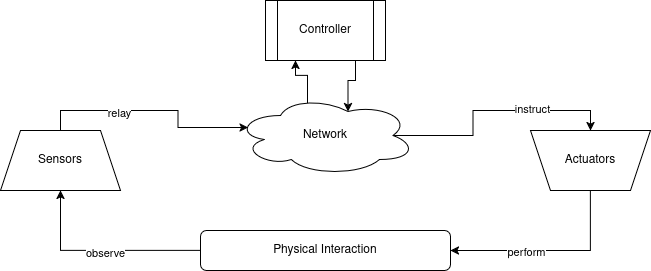
\includegraphics[width=0.7\textwidth]{graphics/cpsGeneralArchitecture.png}
  \caption{General architecture of common CPS}
  \label{fig:cps_architecture}
\end{figure}


Controllers may range from simple reactive routines to advanced inference models grounded in probabilistic programming, or even intelligent agents capable of autonomous
decision-making. Actuators, in turn, translating these decisions into physical action can be represented by basic devices such as motors that move parts, 
valves that regulate flow, or relays that control circuits. They can also act as more complex assemblies — robotic joints, programmable hydraulic systems, or smart actuators 
that adjust based on local conditions. At the foundation, sensors continuously monitor the environment, capturing data through modalities such as motion, 
orientation, or spatial mapping. Together, these elements form  an integrated feedback system, enabling CPS to respond intelligently and flexibly to their physical context,
regardless of application domain.\\

CP-Systems are inherently multidisciplinary structures intersecting engineering domains (mechanical, electrical, civil, etc.) with computer science.
Because these domains employ differing models for ... , effectively combining them is non-trivial. Challenges arise during development and operation of CPSs for which
finding solutions is imperative. \cite{cpsChallengesAndFuture} First and foremost is the concern of \textbf{reliability and safety}. Occurrences of failures can have dire real-world
consequences with catastrophic end results. This means systems must handle unexpected conditions gracefully and robustly. But ensuring safety through extensive verification 
and validation is complicated by the combination of continuous physical dynamics and discrete decision logics. Another challenge is \textbf{real-time performance}, as computing
elements must keep pace with the physical processes, which usually require low-latency responsiveness including the network. Since CPSs are used in infrastructure and other
critical sites that may be targets of cyber attacks, guarantying a high standard of \textbf{Security} is essential. Additionally, sensors are not completely reliable — 
possibly introducing noise to measurements — and environmental conditions can vary drastically leading to \textbf{uncertainty}, which a CPS has to cope with to be resilient. \cite{cpsProbabilisticRobotics}

\section{Formal Methods and Model Checking}

CPSs are often deployed in safety-critical environments where utmost importance is placed on reliable operation and functional correctness. Yet reaching high levels of confidence
in a systems behavior remains extremely inside cyber-physical domains.\cite{formalMethodsCPSCritical} This difficulty arises from the complex interactions of all the individual integral 
components of the system, which can not be effectively tested only employing traditional methods. The inherent entanglement of these systems warrants the use of
specialized procedures that are able to cover and validate the acting components. Unlike conventional simulation based testing, \textit{formal methods} are able to prove correctness against
formal specifications, thereby providing more reliable results and eliminating potential error sources, such as race conditions or violations of safety properties(unnoticed states).

In formal methods, \textit{theorem proving}, \textit{model checking}, and \textit{runtime verification} are widely recognized as the three main approaches for assuring system correctness. \cite{formalMethodsBig3,formalMethodsCPSCritical}
All three practices are distinguishable from one another and are tailored for certain scenarios. Runtime verification is a lightweight technique that verifies systems 
by inspecting their execution trace - often employing automata to detect violations. Theorem proving, in contrast, is an offline and often time intensive 
process relying on mathematical inference rules to statically validate correctness with a high degree of rigor.

Model checking is of most interest to us, as the MiniProb DSL \ref{sec:miniprob} was developed with this context in mind. \cite{THEONEANDONLY1}
Logical Formulas temporal formulas ...
States blabla ... .. 

Model checking is an automated formal verification technique used to exhaustively analyze the behavior of finite-state systems against a formally specified set of 
properties. These properties are typically expressed in temporal logics such as Linear Temporal Logic (LTL) or Computation Tree Logic (CTL), which enable reasoning 
about sequences of states over time (Baier & Katoen, 2008). A model checker systematically explores all reachable states of the system model to verify whether the 
temporal logic specification holds. If a property is violated, the tool provides a counterexample trace, aiding in pinpointing the source of the issue (
  Clarke et al., 1999). The use of logical specifications allows model checking to offer strong correctness guarantees, particularly for safety and liveness 
  properties in reactive and concurrent systems.

\cite{formalMethodsCPSCritical} explains model checking

\section{Motivation for PPLs in CPS Contexts}

Probabilistic programming has multiple fitting applications within CPSs, especially where reasoning under uncertainty is essential. Generally, probabilistic programming
allows controllers to plan even in unpredictable environments and settings.

\begin{multicols}{2}
When measurements contain noise or are incorrect, PPL models can still be applied to extract useful information. Instead of treating the raw reading of a sensor as the “truth,”
the readings are considered samples for a \textit{sensor’s model}. Not only is it possible to reduce the noise in the measurements by calculating the posterior, 
but those noise characteristics are also used to flesh out the predictive model itself.
This enables PPLs to adaptively adjust noise models online when, for example, sensors deteriorate over time.
Additionally — with most CPSs employing multiple sensors — a PPL naturally supports \textit{sensor fusion}, \cite{cpsSensorFusion} combining data from heterogeneous sources
to produce a coherent estimate. By defining each sensor's observation as a conditional distribution, a probabilistic program
weights each reading according to its uncertainty: more reliable sensors contribute more heavily, while inconsistent or faulty readings are down-weighted or flagged. 
Inference then yields a joint posterior over the true state, allowing the system to reconcile disagreements between sensors, detect potential sensor failures by inferring 
latent bias variables, and maintain a quantified confidence.
\\
Which leads us into robotics, a quintessential cornerstone of CPS. Instead of working on raw observational data and making assumptions in incomplete cases, robots can adopt 
a \textit{belief} based on an observational model \cite{cpsProbabilisticRobotics}. The observational model couples motion dynamics (how actions translate into state 
transitions) with existing sensor models, providing a full posterior distribution that the robot can use to imply different levels of confidence for its actions.
Furthermore, robots often operate in changing environments or with components that degrade over time. Within a PPL, unknown parameters, such as friction 
coefficients or sensor calibration offsets, can be treated as latent variables and perform Bayesian learning to infer them from incoming data. The same inference mechanism used for state 
estimation thus also adapts the model online, continuously refining both motion dynamics and sensor mappings.
\\
A PPL expresses system dynamics probabilistically so that sampling yields a distribution of possible futures. \cite{cpsPredictiveControl} By enforcing “chance constraints” 
(e.g., “limit the probability of exceeding a safety threshold to 1\%”), inference or Monte Carlo sampling identifies control inputs that optimize expected performance while 
respecting risk. When the current state is uncertain, planning occurs in belief space — each action triggers a Bayesian update of the state distribution, and planners 
choose sequences that minimize expected cost given that uncertainty. Simultaneously, online Bayesian learning refines model parameters (like friction or drag) over time, 
tightening future predictions; as uncertainty shrinks, control can push closer to limits, whereas rising uncertainty leads to more conservative actions.
\\
Recent research is looking at ways to utilize PPLs to gather diagnostics of a CPS. \cite{cpsPPLDiagnostics} They authors propose a way to infer potential error causes, that
might be overlooked otherwise, due to the . 
This of of great interest to system operators for deciding if either parts have to be replaced or only have to be recelebrated. Because measured data on system deviations
often reflects complex intertwining causes and \textit{closed-loop corrections}, identifying root causes becomes a matter of inference. The proposed two-step approach 
first builds a generative model (based on control software and expert insights) that simulates observations from hypothesized error causes. This simulator is then recast 
as a probabilistic program, allowing Bayesian inference to estimate latent causes (with confidence intervals) from actual measurements.

\end{multicols}

\chapter{Probabilistic Programming}
\section{What Is Probabilistic Programming?}

Probabilistic programming is a paradigm that aims to perform statistical analysis using tools yielded by computer science.\cite{introductionprobabilisticprogramming}
Unifying general-purpose programming and probabilistic modelling enables the presentation of statistical models as a program. Defined by underlying program code, the model is
embodied by the relations between variables and calculations. The established capabilities of programming languages are often augmented with 
probabilistic functionality, in ... creating probabilistic programming languages (PPL),\cite{probProgrammingPrinciples} that are closely associated with this paradigm. 
The enriched syntax enables the creation of more compact models and fosters conciser abstractions of the underlying probabilistic structure, usually providing constructs
that allow declaring random variables and conditioning of observed data, typical for probabilistic modelling. These constructs form the foundation for specifying core elements
of statistical models. \textit{Priors} are pre-known and usually drawn from distributions reflecting the initial belief over what value
\textit{latent variables}/model parameters might take on. \textit{Likelihoods} are also known beforehand representing how data is assumed to be generated given the 
latent variable for which the \textit{posterior} is to be inferred. Together, these components form the backbone of a probabilistic model and provide the information required
to compute the posterior distribution, which is grounded in \textbf{Bayesian theory}.\cite{introductionprobabilisticprogramming}
\\

\textit{Bayes’ Theorem} provides the foundational framework for probabilistic reasoning under uncertainty. It describes how to update prior beliefs about unknown 
quantities - known as latent variables - based on new evidence, resulting in a posterior distribution. Formally, it states that the posterior is proportional to the
product of the prior and the likelihood:
\[
P(\theta \mid x) \propto P(x \mid \theta) \cdot P(\theta)
\]
In probabilistic programming, this principle is applied through models that define prior distributions over latent variables and likelihood functions for 
observed data. The probabilistic programming language then applies Bayes' Theorem, typically via automated inference algorithms, to compute or approximate the posterior.
This makes it possible to express complex probabilistic models declaratively, while delegating the computation of posterior beliefs to the underlying inference engine.
\\

\section{Inference and Sampling Methods}

Inference is the process by which probabilistic models are "executed". Given a model and observed data, the task is to compute the posterior distributions of latent variables.
Because probabilistic models often include uncertainty and hidden variables, inference is the process that turns the model into concrete answers.
This process is abstracted and automated, but remains computationally nontrivial. Standard approaches to inference are generally grouped 
into three main categories- \textit{exact inference}, \textit{sampling-based methods}, and \textit{variational inference}.\cite{bishop2006prml, blei2017vi, goodman2014dippl}.

\subsection*{1. Exact Inference}

Exact inference computes the posterior distribution analytically or through complete enumeration. This is possible only in models with limited complexity where the 
entire state space can be traversed. Although conceptually straightforward, exact inference quickly becomes infeasible as model size increases, due to the combinatorial
explosion of possible states.

\subsection*{2. Sampling-Based Inference}

Sampling-based inference approximates the posterior by drawing samples from it, typically using Markov Chain Monte Carlo (MCMC) methods.
Continuously, random samples are generated from a given distribution - usually the prior or a conditional- and used to progressively approximate
the posterior with the model being executed repeatedly.
These approaches are flexible and can handle complex models, but they are often computationally expensive and require many samples to ensure accuracy.
The resulting samples can then be used to estimate expectations, marginal distributions, or event probabilities.

\subsection*{3. Variational Inference}

Variational inference formulates inference as an optimization problem. Instead of sampling, it produces a family of approximate distributions and seeks the member that 
is closest to the true posterior. This involves defining an objective function - often the \textit{evidence lower bound (ELBO)} - and optimizing it using gradient-based methods.
Variational inference tends to be faster and more scalable than sampling, though it trades off exactness for speed by approximating the posterior rather than sampling
from it directly \cite{blei2017vi}.


\begin{figure}[htbp]
  \centering
  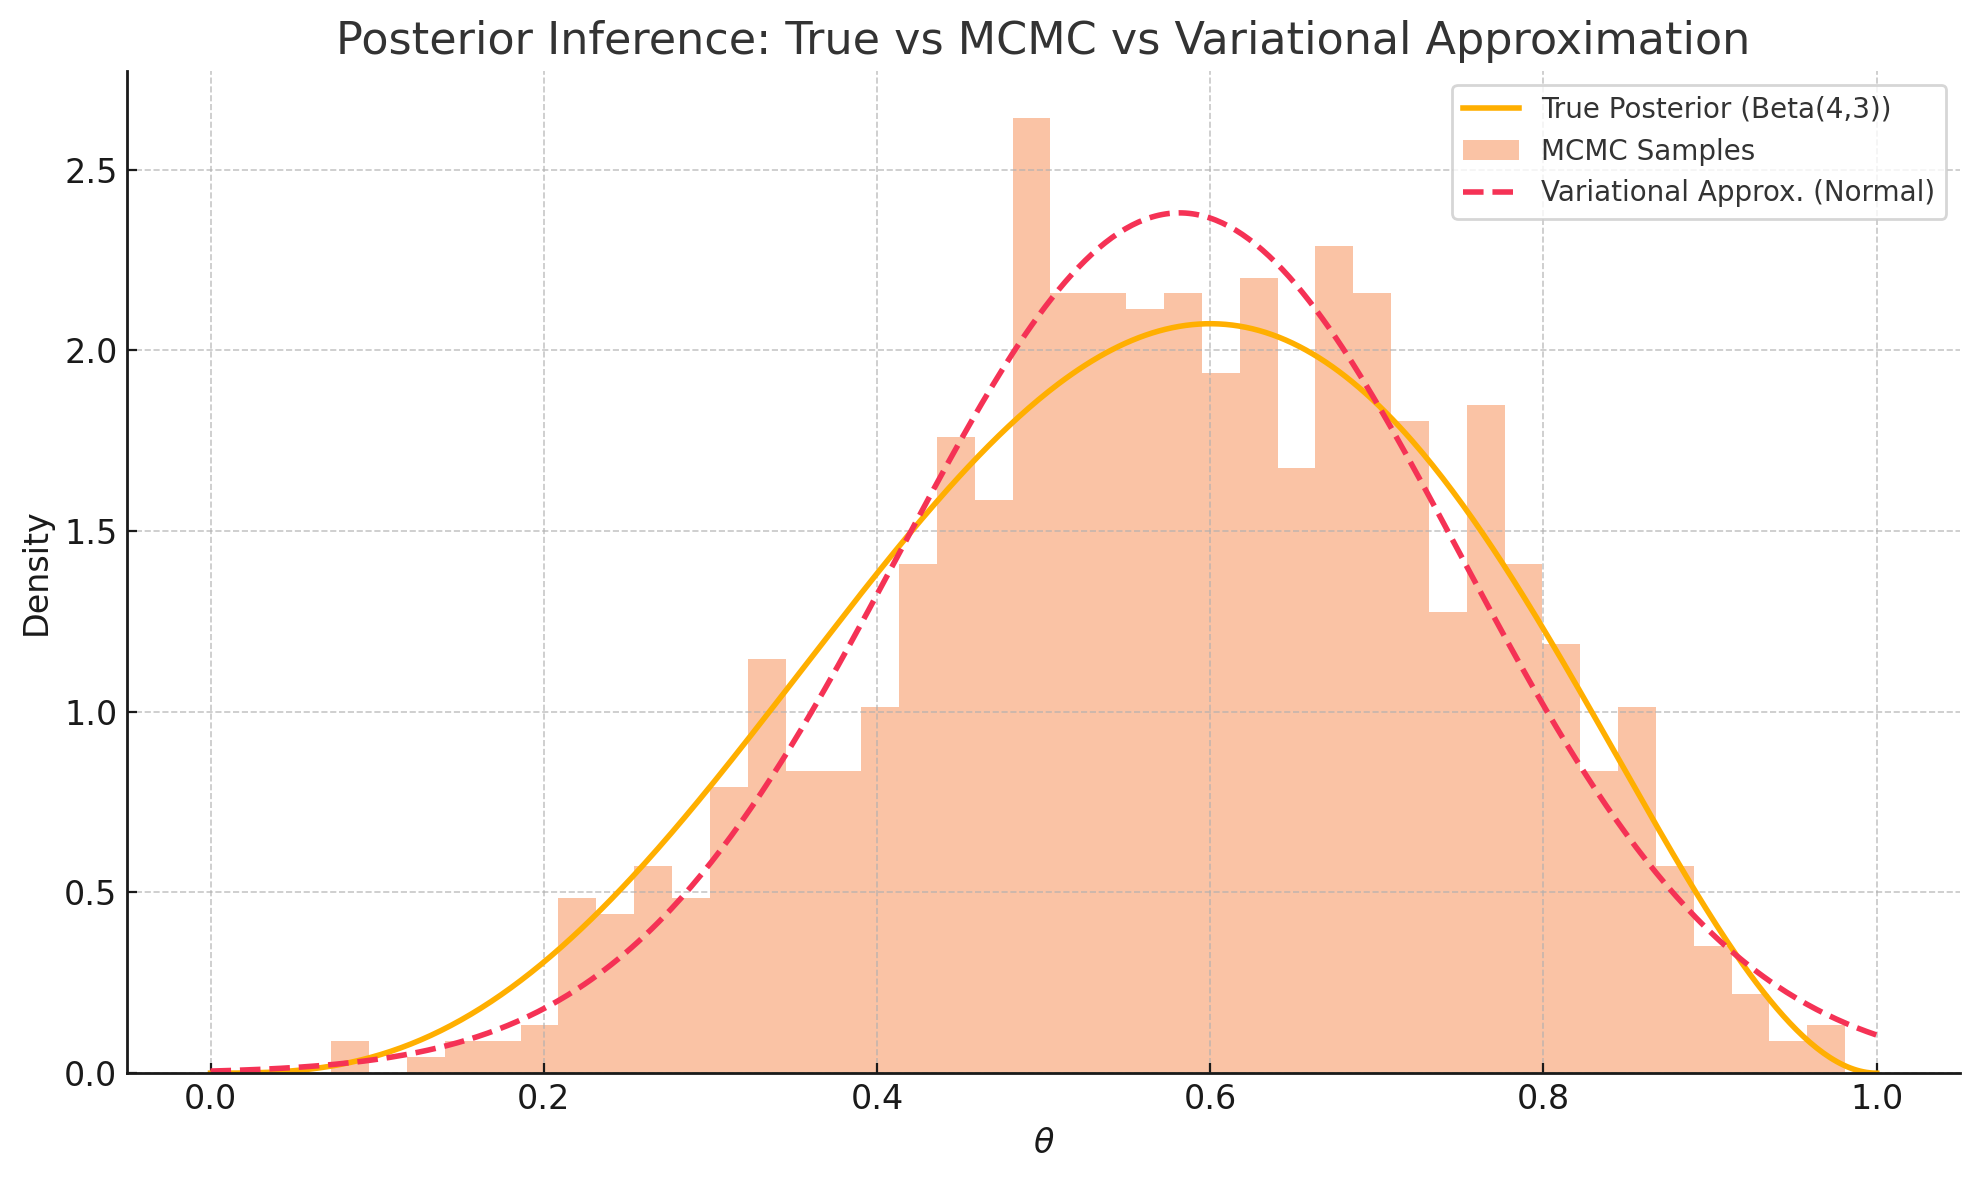
\includegraphics[width=0.7\textwidth]{graphics/inferencePlot.png}
  \caption{Comparison sample of exact posterior to inference methods}
  \label{fig:inference_plot}
\end{figure}

\section{Symbolic Semantics and Model Checking}
pOPA ... ref to CPS Model Checking or put chapter after CPS

Inlcude graphic displaying sampling approximations compared to a symbolic state evaluation

\label{sec:miniprob}
\chapter{The \textit{MiniProb} DSL}
\section{Domain and Purpose}
\section{Syntax Overview}
\section{Semantics and Example Models}

\chapter{Language Servers, Parsers \& Type Checking}
https://code.visualstudio.com/api/language-extensions/overview
\section{Language Server Protocol (LSP) Basics}
\section{Parser and Syntax Checking}
\section{Type Checking Functionality}
\section{Overview of Langium}

%=== Part II – Design \& Implementation ===%
\part{Design \& Implementation}

\chapter{Requirements \& Technology Survey}
\section{Functional Requirements}
\section{Non-functional Requirements}
\section{Alternative Technologies}
\section{Justification for Langium \& VS Code}

\chapter{Architectural Design}
\section{High-Level Architecture Diagram}
\section{Module Decomposition}
\section{Data Flow and Control Flow}

\chapter{Implementation Details}
\label{sec:langium-grammar}
\section{Langium Grammar Definition for \textit{Miniprob}}
\section{Semantic Checks and Type System}
\section{VS Code Extension Points}

\chapter{Testing \& Validation}
\section{Unit Tests}
\section{Integration Tests}
\section{Case Studies \& Examples}

%=== Part III – Evaluation \& Discussion ===%
\part{Evaluation \& Discussion}

\chapter{Performance \& Usability}
\section{Parsing Speed}
\section{Editor Responsiveness}
\section{User Feedback}

\chapter{Discussion}
\section{Meeting the Requirements}

\printbibliography

\appendix

% Full Miniprob grammar here.

\chapter{Expanded Code Listings}
% Additional code excerpts.

\chapter{Test Data}
% Sample inputs, test cases, etc.

\end{document}
